Alternatively, the constrained optimization problem \eqref{eq:YB_isoTPS_YB_move_standard} can be solved via two successive SVDs with an optional disentangling prodcedure with the goal of reducing the truncation error or some entanglement measure. This is is a similar algorithm to the one used for the MM in isoTPS \cite{cite:efficient_simulation_of_dynamics_in_two_dimensional_quantum_spin_systems}, compare Section \ref{sec:tensors_and_tensor_networks_isometric_tensor_product_states_in_2D}. The algorithm is sketched in Figure \figref{fig:yb_move_svd_disent} and is made up of three main steps.
\begin{enumerate}
	\item We start by contracting the tensors $T$, $W_1$ and $W_2$ into a single tensor $\Psi$ at a cost of $\mathcal{O}(\chi^3D^4+\chi^2D^6d) = \mathcal{O}(D^8d)$. This tensor is then split from left to right via a truncated SVD
	\begin{equation}
		\Psi = ASV^\dagger = A(SV^\dagger) \eqqcolon A\theta
	\end{equation}
	as shown in Figure \figref{fig:yb_move_svd_disent_a}. Here, the bond connecting $A$ and $\theta$ has a bond dimension of $\min(dD^2, \chi^2D^2)$. The bond dimension is truncated to $D^2$. The cost of the SVD is $\mathcal{O}(\chi^2D^6d^2) = \mathcal{O}(D^8d^2)$.
	\item Next, we split the index of the bond connecting $A$ and $\theta$ into two indices of dimension $D$ each, see Figure \figref{fig:yb_move_svd_disent_b}. To proceed, we note that there exists a degree of freedom on the bonds connecting $A$ and $\theta$: A unitary $U$ and its adjoint can be inserted as shown in the second step of Figure \figref{fig:yb_move_svd_disent_b} without changing the result of the contraction
	\begin{equation}
		AU^\dagger U\theta = (AU^\dagger)(U\theta) \eqqcolon T^\prime \tilde{\theta}.
	\end{equation}
	The unitary $U$ can be chosen to minimize the truncation error of the next step by \textit{disentangling} the tensor $\theta$. We will discuss procedures of finding such a \textit{disentangling unitary} $U$ on the next page.
	\item In the last step, the tensor $\tilde{\theta}$ is split vertically into $W_1^\prime$ and $W_2^\prime$ using a truncated SVD as shown in Figure \figref{fig:yb_move_svd_disent_c}. The computational cost of this SVD scales as $\mathcal{O}(\chi^3D^6) = \mathcal{O}(D^9)$. Here, the bond dimension is truncated to $\chi$. We end up with the three tensors $T^\prime$, $W_1^\prime$ and $W_2^\prime$, completing the YB move.
\end{enumerate}
Before we discuss the disentangling procedure, two comments about step two of the above algorithm are in order. First, there exists a degree of freedom for splitting the bond index, because applying the same permutations to the columns of $A$ and rows of $\theta$ does not change the result of contracting the network. However, this degree of freedom is fixed by the disentangling process, making the exact permutation of the bond splitting irrelevant. Second, note that near the edges of the lattice it can happen that the matrixized tensor $\Psi$ has $\tilde{\chi} < D^2$ rows. In this case, the bond dimension after the SVD will also be $\tilde{\chi}$ and we cannot simply split the bond into two bonds of dimension $\chi_1=\chi_2=D$. Instead, we choose a splitting $\chi_1 \le D$, $\chi_2 \le D$ such that $\chi_1\cdot\chi_2$ is maximized, while it must still hold $\chi_1\cdot\chi_2\le\tilde{\chi}$. We additionally prefer "equal" splittings $\chi_1\approx\chi_2\approx\sqrt{\tilde{\chi}}$ if possible. One can find such a splitting easily by computing all possible combinations of $\chi_1$ and $\chi_2$ and keeping only the best one, which has a computational cost of $\mathcal{O}\left(\sqrt{\tilde{\chi}}\right) = \mathcal{O}\left(D\right)$. See also our implementation at \cite{cite:github_YB_isoTPS}.\par
\begin{figure}
	\centering
	\subcaptionbox{\label{fig:yb_move_svd_disent_a}}
	{%
		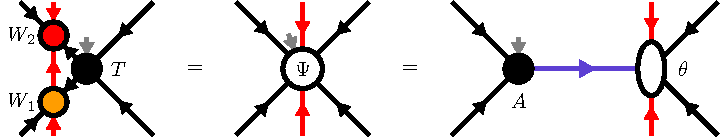
\includegraphics[scale=1.0]{figures/tikz/YB_isoTPS/yang_baxter_move_svd/yang_baxter_move_svd_a.pdf}
	}
	\par\bigskip
	\subcaptionbox{\label{fig:yb_move_svd_disent_b}}
	{%
		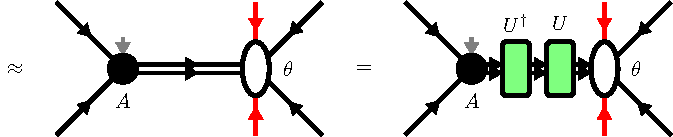
\includegraphics[scale=1.0]{figures/tikz/YB_isoTPS/yang_baxter_move_svd/yang_baxter_move_svd_b.pdf}
	}
	\par\bigskip
	\subcaptionbox{\label{fig:yb_move_svd_disent_c}}
	{%
		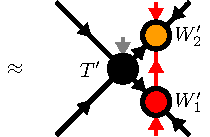
\includegraphics[scale=1.0]{figures/tikz/YB_isoTPS/yang_baxter_move_svd/yang_baxter_move_svd_c.pdf}
	}
	\caption{The YB move is made up of three steps as explained in the text.}
	\label{fig:yb_move_svd_disent}
\end{figure}
\subsubsection*{\hspace{132pt}The disentangling process}
We will now discuss the problem of finding a good disentangling unitary $U$ for step 2 of the above algorithm, which is crucial for the performance of the YB move. The problem can be formulated as follows: Given the tensor $\theta$ that is obtained after splitting the index in step two, find a unitary $U$ minimizing a cost function $f(U, \theta)$. In the following, let $\tilde{\theta}_{(l,i),(j,r)}$ be the $\chi D^2\times \chi D^2$ matrix that is obtained by reshaping the contraction $\tilde{\theta}_{l,i,j,r} = \sum_{i^\prime,j^\prime} U_{i,j,i^\prime,j^\prime}\theta_{l,i^\prime,j^\prime,r}$ into a matrix as shown in Figure \figref{fig:disentangling_theta_definition}. Let further $\tilde{\theta} = XSY^\dagger$ denote the SVD of $\tilde{\theta}$. We discuss two cost functions, as also done in \cite{cite:effefficient_simulation_of_dynamics_in_two_dimensional_quantum_spin_systems}. The first cost function is simply given by the truncation error
\begin{equation}
	\label{eq:YB_move_disent_cost_function_truncation_error}
	f_\text{trunc}\left(U,\theta\right) = \sqrt{\sum_{\mu = \chi+1}^{\chi D^2}S_\mu^2}
\end{equation}
arising in step three of the YB move. Alternatively, one can think of $|\tilde{\theta}\rangle \coloneqq \sum_{(l,i), (j,r)}\tilde{\theta}_{(l,i),(j,r)}\ket{(l,i), (j, r)}$ as a bipartite state in an orthogonal basis and consider as a cost function the Rényi-entropy
\begin{equation}
	\label{eq:renyi_entropy}
	f_\text{Rényi}\left(U,\theta,\alpha\right) = \frac{1}{1-\alpha}\log\Tr\left(\rho^\alpha\right) = \frac{1}{1-\alpha}\log\left(\sum_{\mu=1}^{\chi D^2}S_\mu^{2\alpha}\right),
\end{equation}
where $\alpha\in[0,\infty)$ and $\rho = \Tr_{(j, r)}(\ket{\tilde{\theta}}\bra{\tilde{\theta}})$ is the reduced density matrix obtained by tracing out one of the subsystems, see Figure \figref{fig:disentangling_rho_definition}. In the last step of \eqref{eq:renyi_entropy} we used the fact that the eigenvalues of $\rho$ are the squares of the singular values of $\tilde{\theta}$. The Rényi-entropy can be used as a measure of entanglement. It approaches the Von-Neumann entanglement entropy for $\alpha\rightarrow 1$. It can be shown that the truncation error is bounded by the Rényi-entropy if $\alpha < 1$ \cite{cite:mps_represent_ground_states_faithfully}, which is a motivation for using $f_\text{Rényi}$ as a cost function. For $\alpha > 1$ such a bond cannot generally be given. However, optimizations of Rényi-entropies with $\alpha > 1$ are often simpler to perform and still achieve good results in practice \cite{cite:isometric_tensor_network_states_in_two_dimensions, cite:efficient_simulation_of_dynamics_in_two_dimensional_quantum_spin_systems, cite:finding_purifications_with_minimal_entanglement}. Setting $\alpha = 2$ yields the Rényi-entropy
\begin{equation}
	\label{eq:renyi_entropy_alpha_2}
	f_\text{Rényi}\left(U,\theta,\alpha=2\right) = -\log\Tr\rho^2,
\end{equation}
which can easily computed by contracting the tensor network shown in Figure \figref{fig:disentangling_evenbly_vidal_algorithm_trace_rho_squared} without needing to perform an SVD \cite{cite:finding_purifications_with_minimal_entanglement}. The cost function $f_\text{Rényi}\left(U,\theta,\alpha=2\right)$ can be minimized using the Evenbly-Vidal algorithm as proposed in \cite{cite:finding_purifications_with_minimal_entanglement}. First, we rewrite the minimization problem as a maximization problem
\begin{equation}
	U_\text{opt} = \underset{U^\dagger U = \id}{\argmin} f_\text{Rényi}\left(U,\theta,\alpha=2\right) = \underset{U^\dagger U = \id}{\argmax}\Tr\rho^2.
\end{equation}
We proceed by taking one tensor $U$ out of the network $\Tr\rho^2$ and contracting all other tensors into the environment $E$ as shown in Figure \figref{fig:disentangling_evenbly_vidal_algorithm_environment_definition}. We now treat $E$ as if it were independent of $U$ and update $U\leftarrow AB^\dagger$, where $A$ and $B$ are obtained by taking the SVD $E=A\Lambda B^\dagger$. This is repeated until convergence. For details on the Evenbly-Vidal algorithm see Appendix \ref{sec:evenbly_vidal_algorithm}. In practice it is observed that this algorithm for minimizing $f_\text{Rényi}\left(U,\theta,\alpha=2\right)$ converges very quickly \cite{cite:efficient_simulation_of_dynamics_in_two_dimensional_quantum_spin_systems}. The computational cost of this algorithm is dominated by the contraction of the effective environment $E$, which scales as $\mathcal{O}(\chi^3D^6) = \mathcal{O}(D^9)$. The full cost of the algorithm is thus $\mathcal{O}(N_\text{iter}D^9)$, with $N_\text{iter}$ the number of disentangling iterations.\par
\begin{figure}
	\centering
	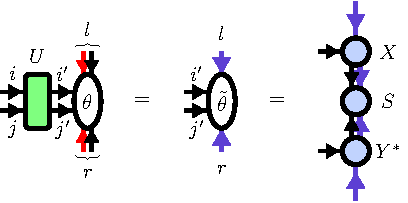
\includegraphics[scale=1]{figures/tikz/YB_isoTPS/theta_tilde_contraction/theta_tilde_contraction.pdf}
	\caption{The disentangling unitary $U$ is contracted with the wave function tensor $\theta$ to form $\tilde{\theta}$, which is subsequently split via an SVD $\tilde{\theta} = XSY^\dagger$. The purple legs have bond dimension $\chi D$.}
	\label{fig:disentangling_theta_definition}
\end{figure}
\begin{figure}
	\centering
	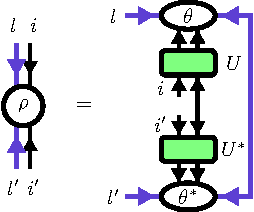
\includegraphics[scale=1]{figures/tikz/YB_isoTPS/rho_definition/rho_definition.pdf}
	\caption{Definition of the reduced density matrix $\rho$. The purple legs have bond dimension $\chi D$.}
	\label{fig:disentangling_rho_definition}
\end{figure}
\begin{figure}
	\centering
	\subcaptionbox{\label{fig:disentangling_evenbly_vidal_algorithm_trace_rho_squared}}
	{%
		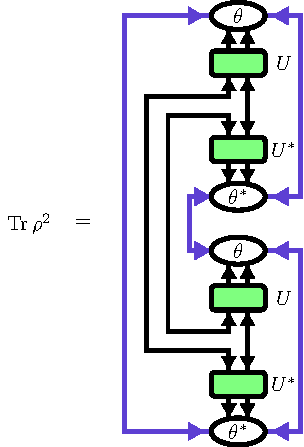
\includegraphics[scale=1]{figures/tikz/YB_isoTPS/evenbly_vidal_renyi_2/evenbly_vidal_renyi_2_a.pdf}
	}
	\quad\quad\quad\quad
	\subcaptionbox{\label{fig:disentangling_evenbly_vidal_algorithm_environment_definition}}
	{%
		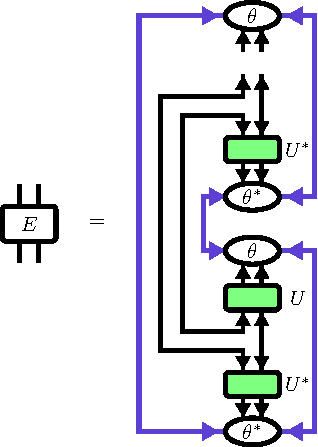
\includegraphics[scale=1]{figures/tikz/YB_isoTPS/evenbly_vidal_renyi_2/evenbly_vidal_renyi_2_b.pdf}
	}
	\caption{(a) Tensor network for the computation of the cost function \eqref{eq:renyi_entropy_alpha_2}. (b) Taking out one unitary $U$, the tensor network is contracted into the environment $E$.}
	\label{fig:disentangling_evenbly_vidal_algorithm}
\end{figure}
\begin{figure}
	\centering
	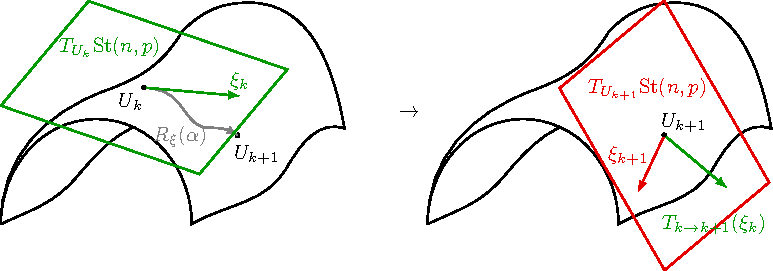
\includegraphics[scale=1]{figures/tikz/YB_isoTPS/riemannian_optimization/riemannian_optimization.pdf}
	\caption{In this figure, a visualization of optimization on Riemannian manifolds is given. The iterate $U_k$ (left) is updated along the search direction $\xi_k$, which is an element of the tangent space $T_{U_k}\Stiefel$. The next iterate $U_{k+1}$ is computed with the retraction $R_\xi\left(\alpha\right)$, where $\alpha\in\mathbb{R}$ is the step size. For the computation of the next search direction $\xi_{k+1}$ some algorithms need the previous search direction $\xi_k$, which must first be brought to the tangent space $T_{U_{k+1}}\Stiefel$ of the new iterate $U_{k+1}$ via the vector transport $T_{k\rightarrow k+1}\left(\xi_k\right)$.}
	\label{fig:disentangling_riemannian_optimization}
\end{figure}
Minimizing the truncation error $f_\text{trunc}\left(U,\theta\right)$ and general Rényi-entropies $f_\text{Rényi}\left(U,\theta,\alpha\neq2\right)$ is a harder problem. We follow the approach of \cite{cite:isometric_tensor_network_states_in_two_dimensions, cite:efficient_simulation_of_dynamics_in_two_dimensional_quantum_spin_systems} and use Riemannian optimization \cite{cite:optimization_on_matrix_manifolds, cite:optimization_techniques_on_riemannian_manifolds, cite:riemannian_optimization_isometric_tensor_networks, cite:riemannian_geometry_automatic_differentiation_quantum_physics, cite:pymanopt} to solve the optimization problem. The idea of Riemannian optimization is to generalize common optimization algorithms that are defined in Euclidian vector spaces, such as Gradient Descent or Conjugate Gradients, to Riemannian manifolds. The set of all isometric matrices of shape $n\times m$ is a Riemannian manifold called the Stiefel manifold $\Stiefel$. A special case is the set of all unitary matrices of shape $n\times n$, $U(n)=\text{St}(n, n)$, over which we want to optimize here. Riemannian optimization over the Stiefel manifold is discussed in more detail in Appendix \ref{app:riemannian_optimization_of_isometries}. \par
A typical optimization algorithm iteratively improves an iterate $U_k\in\Stiefel$, $k=1,2,\dots$ until a local minimum of the cost function $f$ is found. In Riemannian optimization, the gradient of the cost function $\nabla f\left(U_k\right)$ is restricted to the tangent space $T_{U_k}\Stiefel$ of the iterate $U_k$ \cite{cite:optimization_on_matrix_manifolds}, which we visualize in Figure \figref{fig:disentangling_riemannian_optimization}. The gradient can be computed either analytically or via automatic differentiation \cite{cite:riemannian_geometry_automatic_differentiation_quantum_physics, cite:pymanopt}. Optimization algorithms typically compute a search direction $\xi_k\in T_{U_k}\Stiefel$ and a step size $\alpha_k \in \mathbb{R}$ from the gradient. In an optimization algorithm defined on an Euclidean vector space one would then move along this direction as
\begin{equation}
	\tilde{U}_{k+1} = U_k + \alpha_k\xi_k.
\end{equation}
However, $\tilde{U}_{k+1}$ is in general not an element of the manifold. To ensure $U_{k+1}\in\Stiefel$, one can introduce a \textit{retraction} $R_{\xi_k}:\mathbb{R}\to\Stiefel$ \cite{cite:optimization_on_matrix_manifolds}. One can think of $R_{\xi_k}(\alpha_k)$ as moving along the direction of $\xi_k$ while staying on the manifold. As $\alpha_k$ increases, we move further along the path defined by the retraction, with $R_{\xi_k}(0) = U_k$, see Figure \figref{fig:disentangling_riemannian_optimization}. Different retractions can be chosen, varying by how well they perform in optimization problems and by how hard they are to compute. Here we choose the retraction
\begin{equation}
	R_{\xi_k}(\alpha_k) = \qf\left(U_k + \alpha_k\xi_k\right),
\end{equation}
where $\qf\left(A\right)$ is the Q-factor of the QR-decomposition $A = QR$. This retraction is particularly easy to compute and yields good results in practice. \par
Many optimization algorithms such as Conjugate Gradients require gradients or search directions from previous iterates for computing a search direction at the current iterate. In Riemannian optimization, one must first bring these gradients and search directions from the tangent spaces of previous iterates to the tangent space of the current iterate. This is handled by a so-called \textit{vector transport} $T_{k\rightarrow k+1}\left(\xi_k\right)$ \cite{cite:optimization_on_matrix_manifolds}, see Figure \figref{fig:disentangling_riemannian_optimization}. \par
Finally, for optimization algorithms of second order such as the trust-region method, one needs to generalize the notion of the hessian-vector product to Riemannian manifolds. This generalization is given by the \textit{Riemannian connection} \cite{cite:optimization_on_matrix_manifolds}. For the Stiefel manifold the hessian-vector product is simply given by projecting the hessian vector product of the embedding euclidean vector space $\mathbb{C}^{n\times p}$ to the tangent space. \par
We use two algorithms for solving the disentangling optimization problem, Conjugate Gradients (CG) and the Trust-Region Method (TRM). CG uses the accumulated gradients of previous iterations to compute an improved search direction, trying to achieve superlinear convergence. CG is discussed in more details in Appendix \ref{sec:conjugate_gradients}. The TRM approximates the cost function around the current iterate through a quadratic function using the hessian vector product. This approximate cost function is then minimized within a region of radius $\Delta\in\mathbb{R}$ using truncated Conjugate Gradients (tCG), which converges quickly for the quadratic approximation. Depending on the quality of the approximation at the current iterate one can then shrink or enlarge the trust region. TRM is able to achieve local superlinear convergence while still retaining desired global convergence properties \cite{cite:optimization_on_matrix_manifolds} and can be thought of as an improved version of Newton's method. For more details, see Appendix \ref{sec:trust_region_method}. \par
The gradients and hessian vector products of the cost functions \eqref{eq:YB_move_disent_cost_function_truncation_error} and \eqref{eq:renyi_entropy} can be computed analytically with a computational cost of $\mathcal{O}(D^9)$, see Appendix \ref{app:computation_of_gradient_and_hvp_for_riemannian_optimization} for a derivation.
\subsubsection*{\hspace{70pt}Approximate gradients and hessian vector products}
\begin{figure}
	\centering
	\subcaptionbox{\label{fig:approximate_svd_overlap}}
	{%
		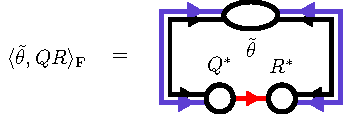
\includegraphics[scale=1]{figures/tikz/YB_isoTPS/approximate_svd/approximate_svd_a.pdf}
	}
	\par\bigskip
	\subcaptionbox{\label{fig:approximate_svd_first_step}}
	{%
		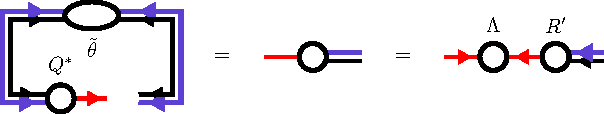
\includegraphics[scale=1]{figures/tikz/YB_isoTPS/approximate_svd/approximate_svd_b.pdf}
	}
	\par\bigskip
	\subcaptionbox{\label{fig:approximate_svd_second_step}}
	{%
		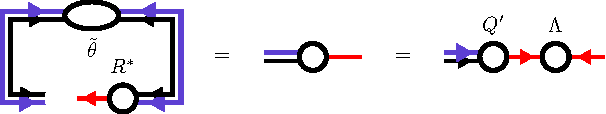
\includegraphics[scale=1]{figures/tikz/YB_isoTPS/approximate_svd/approximate_svd_c.pdf}
	}
	\par\bigskip
	\subcaptionbox{\label{fig:approximate_svd_final_step}}
	{%
		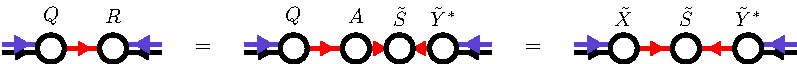
\includegraphics[scale=1]{figures/tikz/YB_isoTPS/approximate_svd/approximate_svd_d.pdf}
	}
	\caption{In this figure we draw tensor diagrams for the approximate SVD. First, an approximate QR-decomposition is performed by minimizing the inner product $\langle\tilde{\theta},QR\rangle_\text{F}$ (a). This can be done by iteratively updating the $R$-tensor (b) and the $Q$-tensor (c). We finish the approximate SVD by performing a standard SVD on the tensor $\Lambda$, which has reduced bond dimension (d).}
	\label{fig:approximate_qr_decomposition}
\end{figure}
The cost of both CG and the TRM are dominated by the computation of the gradient and hessian vector product, particularly by the SVD $\tilde{\theta} = XSY^\dagger$ and contractions involving the tensors $X$ and $Y$. The reason for this is the large bond dimension $\chi D^2$ of the bond connecting $X$ and $Y$, see Figure \ref{fig:disentangling_theta_definition}. We thus propose to approximate the gradient and hessian vector product by instead performing an approximate SVD $\tilde{\theta} \approx \tilde{X}\tilde{S}\tilde{Y}^\dagger$, where we only keep $\chi$ of the $\chi D^2$ singular values. The algorithm for performing this approximate SVD is inspired by \cite{cite:fast_time_evolution_of_mps_using_qr}, where a similar algorithm was used to speed up TEBD updates for MPS. We sketch the algorithm in Figure \figref{fig:approximate_qr_decomposition}. First, an approximate QR-decomposition $\tilde{\theta} = QR$ with $Q\in\mathbb{C}^{\chi D^2\times\chi}$ and $R\in\mathbb{C}^{\chi\times\chi D^2}$ is performed by variationally minimizing the distance $\lVert \tilde{\theta} - QR \rVert$, which is equivalent to maximizing the real part of the overlap $\Re\langle\tilde{\theta},QR\rangle_\text{F}$. The overlap is shown as a tensor diagram in Figure \figref{fig:approximate_svd_overlap}. It can be maximized by alternatingly optimizing the tensors $Q$ and $R$ as shown in figures \figref{fig:approximate_svd_first_step} and \figref{fig:approximate_svd_second_step} respectively, which costs $\mathcal{O}(\chi^3D^4) = \mathcal{O}(D^7)$ per iteration. A standard SVD is then performed on the $R$-factor of the approximate QR-decomposition as $R = A\tilde{S}\tilde{Y}$, and the contraction $\tilde{X} = QA$ finalizes the decomposition, see Figure \figref{fig:approximate_svd_final_step}. In total, the cost of the approximate SVD is $\mathcal{O}(N_\text{svd}D^7)$, with $N_\text{svd}$ the number of iterations, instead of $\mathcal{O}(D^9)$ for a full SVD. It is observed that the variational minimization that is used to compute the approximate SVD converges very quickly in practice, especially if a good initialization is chosen. As the iterates $U_k$ are expected to only change slightly in each iteration of CG or TRM, one can simply use the result $Q, R$ obtained in the approximate QR-decomposition of the previous iteration as initialization for the next iteration. We observe that the variational optimization in practice converges in less than $5$ iterations. \par
Using the approximate SVD, we were able to decrease the cost of the gradient computation from $\mathcal{O}(D^9)$ to $\mathcal{O}(D^8 + N_\text{svd}D^7)$. Moreover, through cashing of the most costly contraction, the cost of the tCG sub procedure that is called in every iteration of the TRM can be brought down from $\mathcal{O}(N_\text{tCG}D^9)$ to $\mathcal{O}(D^8+N_\text{svd}D^7 + N_\text{tCG} D^7)$, where $N_\text{tCG}$ is the maximum number of iterations for which the tCG sub procedure is run. Finally, one can also use an approximate SVD for the final vertical splitting performed in step three of the YB move after the disentangling is complete, improving the scaling from $\mathcal{O}(D^9)$ to $\mathcal{O}(N_\text{svd}D^7)$. To summarize, we list the computational complexity of all discussed algorithms for the YB move in Table \figref{table:computational_complexity_YB_move}.
\begin{table}
	\begin{tabular}{ l | l }
		Evenbly-Vidal style iterative optimization & $\mathcal{O}(N_\text{iter}D^8)$ \\ \\[-1em]
		\hline \\[-1em]
		SVD splitting & $\mathcal{O}(D^9)$ \\ \\[-1em]
		\hline \\[-1em]
		approximate SVD splitting & $\mathcal{O}(D^8 + N_\text{svd}D^7)$ \\ \\[-1em]
		\hline
		\hline \\[-1em]
		Evenbly-Vidal Rényi-2 disentangler  & $\mathcal{O}(N_\text{iter}D^9)$ \\ \\[-1em]
		\hline \\[-1em]
		CG disentangler & $\mathcal{O}(N_\text{iter}D^9)$ \\ \\[-1em]
		\hline \\[-1em]
		TRM disentangler & $\mathcal{O}(N_\text{iter}N_\text{tCG}D^9)$ \\ \\[-1em]
		\hline \\[-1em]
		approximate CG disentangler & $\mathcal{O}(N_\text{iter}(D^8 + N_\text{svd}D^7))$ \\ \\[-1em]
		\hline \\[-1em]
		approximate TRM disentangler & $\mathcal{O}(N_\text{iter}(D^8 + N_\text{svd}D^7 + N_\text{tCG}D^7))$ \\
	\end{tabular}
	\caption{In this table we summarize the complexity scaling of the different discussed algorithms for performing the YB move. The scaling of the Rényi-entropy and truncation error disentangling is the same, but with different prefactors.}
	\label{table:computational_complexity_YB_move}
\end{table}
\subsubsection*{\hspace{105pt}Comparison of different disentanglers}
We will now compare the different algorithms for solving the disentangling problem.
\begin{figure}
	\centering
	\begin{tikzpicture}[scale=1, trim axis left, trim axis right]
		\begin{axis}[xlabel=$N_\text{iters}$, ylabel={$f_\text{Rényi}(U,\theta,\alpha=2)$}, grid=both, grid style={gray!20}, every axis plot/.append style={very thick}, scale only axis, height=\singleFigureHeight, width=\singleFigureWidth, title={Rényi entropy $\alpha = 2$}]
			
			\addplot[color = 5blue4, mark=*]
			table[x=N_iters, y=f_Renyi_evenbly_vidal, col sep=space]{figures/plots/disoTPS/data/evenbly_vidal_renyi_2_disentangling.txt};
			%\addlegendentry{Evenbly-Vidal}
			
		\end{axis}
	\end{tikzpicture}
	\caption{\todo{Caption}}
	\label{fig:disoTPS_disentangling_evenbly_vidal_renyi_2}
\end{figure}
\begin{figure}
	\centering
	\subcaptionbox{\label{fig:a}}
	{%
		\begin{tikzpicture}[scale=1, trim axis left, trim axis right]
			\begin{axis}[xlabel=$N_\text{iters}$, ylabel={$f_\text{Rényi}(U,\theta,\alpha=1/2)$}, grid=both, every axis plot/.append style={very thick}, scale only axis, height=\doubleVerticalFigureHeight, width=\doubleVerticalFigureWidth, title={Rényi entropy $\alpha = 1/2$}, xtick={0, 200, 400, 600, 800, 1000}, xticklabels={$0$, $200$, $400$, $600$, $800$, $1000$}]
				
				\addplot[color = 5orange4]
				table[x=N_iters, y=f_Renyi_cg, col sep=space]{figures/plots/disoTPS/data/renyi_0.5_entropy_disentangling.txt};
				\addlegendentry{CG}
				
				\addplot[color = 5orange4, dashed]
				table[x=N_iters, y=f_Renyi_approx_cg, col sep=space]{figures/plots/disoTPS/data/renyi_0.5_entropy_disentangling.txt};
				\addlegendentry{approx CG}
				
				\addplot[color = 5green4]
				table[x=N_iters, y=f_Renyi_trm, col sep=space]{figures/plots/disoTPS/data/renyi_0.5_entropy_disentangling.txt};
				\addlegendentry{TRM}
				
				\addplot[color = 5green4, dashed]
				table[x=N_iters, y=f_Renyi_approx_trm, col sep=space]{figures/plots/disoTPS/data/renyi_0.5_entropy_disentangling.txt};
				\addlegendentry{approx TRM}
				
			\end{axis}
		\end{tikzpicture}
	}
	\subcaptionbox{\label{fig:b}}
	{%
		\begin{tikzpicture}[scale=1, trim axis left, trim axis right]
			\begin{axis}[xlabel=$N_\text{iters}$, ylabel={$f_\text{trunc}(U,\theta)$}, grid=both, every axis plot/.append style={very thick}, scale only axis, height=\doubleVerticalFigureHeight, width=\doubleVerticalFigureWidth, title={Truncation error}, xtick={0, 200, 400, 600, 800, 1000}, xticklabels={$0$, $200$, $400$, $600$, $800$, $1000$}]
				
				\addplot[color = 5orange4]
				table[x=N_iters, y=f_trunc_cg, col sep=space]{figures/plots/disoTPS/data/renyi_truncation_error_disentangling.txt};
				\addlegendentry{CG}
				
				\addplot[color = 5orange4, dashed]
				table[x=N_iters, y=f_trunc_approx_cg, col sep=space]{figures/plots/disoTPS/data/renyi_truncation_error_disentangling.txt};
				\addlegendentry{approx CG}
				
				\addplot[color = 5green4]
				table[x=N_iters, y=f_trunc_trm, col sep=space]{figures/plots/disoTPS/data/renyi_truncation_error_disentangling.txt};
				\addlegendentry{TRM}
				
				\addplot[color = 5green4, dashed]
				table[x=N_iters, y=f_trunc_approx_trm, col sep=space]{figures/plots/disoTPS/data/renyi_truncation_error_disentangling.txt};
				\addlegendentry{approx TRM}
				
			\end{axis}
		\end{tikzpicture}
	}
\end{figure}
For this comparison we select the YB move environment $\left\{W_1, W_2, T\right\}$ that was already used to discuss the convergence behaviour of iterative algorithm in Section \ref{sec:YB_move_iterative_local_optimization}. The results on other YB environments agree qualitatively with the results we present here. The bond dimensions chosen for the YB-isoTPS are $D = 4$, $\chi = 24$. \par
We first test the Evenbly-Vidal algorithm optimizing the Rényi-entropy with $\alpha = 2$, see Figure \figref{fig:YB_isoTPS_disentangling_evenbly_vidal_renyi_2}. The algorithm converges very quickly after only $\approx 20$ iterations. The convergence speed depends drastically on the initialization of the disentangling unitary. We find that a initialization based on an SVD of $\theta$ works best, see our implementation \cite{cite:github_YB_isoTPS}. This initialization procedure was introduced for the MM for isoTPS \cite{cite:isometric_tensor_network_states_in_two_dimensions, cite:efficient_simulation_of_dynamics_in_two_dimensional_quantum_spin_systems}. \par
Next we look at the performance of CG and TRM optimizing the Rényi-entropy with $\alpha = 1/2$ and the truncation error in figures \figref{fig:YB_isoTPS_disentangling_cg_trm_renyi_0.5} and \figref{fig:YB_isoTPS_disentangling_cg_trm_truncation_error} respectively. In both cases we observe that the TRM leads to a faster decrease in the cost function for the same number of iterations compared to CG. Remarkably, the approximate versions of both CG and TRM perform almost as good as their exact counterparts. Again, the speed of convergence depends strongly on the initialization. Because of the quick convergence of the Evenbly-Vidal algorithm optimizing the $\alpha = 2$ Rényi-entropy we choose its result as an initialization for the optimization algorithms using Riemannian optimization. This achieved the best results in our testing. \par
Lastly we plot the cost function against the walltime of the algorithms in figures \figref{fig:YB_isoTPS_disentangling_cg_trm_renyi_0.5_walltime} and \figref{fig:YB_isoTPS_disentangling_cg_trm_truncation_error_walltime}. For this benchmark, the algorithms were run on a i5-12500 CPU with 6 cores. As one can see, the approximate versions of both CG and TRM run up to an order of magnitude faster while still providing a comparable minimization of the cost function. Thus, in practice, it is often better to choose a larger maximum bond dimension with the approximate disentangling algorithms instead of a smaller maximum bond dimension with the exact algorithms.
